\section{Results}
\label{sec:results}

\subsection{Main Experiment: LLM Embedding Streams}
\label{sec:main_results}

\Tabref{tab:main_results} presents the mean AUC across all four drift scenarios (abrupt topic, gradual topic, geometric, style shift), averaged over three seeds. Statistical methods---centroid shift, covariance shift, and MMD---achieve perfect detection (AUC\,=\,1.0) with zero detection delay across all scenarios. Among TDA methods, Wasserstein H0 performs best with mean AUC\,=\,0.713, followed by PE-H1 (0.624) and Betti AUC (0.580). The kNN baseline achieves 0.711, comparable to the best TDA method.

\begin{table}[t]
    \centering
    \caption{Mean detection performance across all drift scenarios (3 seeds). Best results per column in \textbf{bold}. Statistical methods achieve perfect AUC on natural topic drift, while TDA methods show moderate sensitivity.}
    \resizebox{\textwidth}{!}{%
    \begin{tabular}{@{}llcccc@{}}
        \toprule
        \textbf{Method} & \textbf{Type} & \textbf{AUC} & \textbf{Delay} & \textbf{FPR} & \textbf{Runtime/win} \\
        \midrule
        Centroid Shift & Statistical & \textbf{1.000} & \textbf{0.0} & 0.10 & \textbf{0.0001s} \\
        Covariance Shift & Statistical & \textbf{1.000} & \textbf{0.0} & 0.10 & 0.24s \\
        MMD (RBF) & Statistical & \textbf{1.000} & \textbf{0.0} & 0.10 & 0.13s \\
        kNN Distance & Statistical & 0.711 & 2.0 & 0.10 & 0.031s \\
        \midrule
        Wasserstein H0 & TDA & \textbf{0.713} & 3.5 & 0.10 & 0.002s \\
        PE-H1 & TDA & 0.624 & 4.5 & 0.10 & $<$0.001s \\
        Betti AUC & TDA & 0.580 & 4.6 & 0.10 & 0.037s \\
        PHD & TDA & 0.518 & 5.4 & 0.10 & 0.057s \\
        PE-H0 & TDA & 0.494 & 6.5 & 0.10 & 0.037s \\
        \bottomrule
    \end{tabular}
    }
    \label{tab:main_results}
\end{table}

\para{Per-scenario breakdown.}
\Tabref{tab:per_scenario} shows AUC for each drift scenario. The three dominant statistical methods achieve AUC\,=\,1.0 uniformly. Among TDA methods, performance varies substantially across scenarios: Wasserstein H0 reaches 0.927 on abrupt topic drift---its best performance---but drops to 0.557 on style shift. The ``Best TDA'' column reports the highest AUC among all TDA methods for each scenario, showing that different TDA features excel on different drift types.

\begin{table}[t]
    \centering
    \caption{Per-scenario AUC (mean over 3 seeds). ``Best TDA'' reports the highest AUC among all five TDA methods for each scenario. Statistical methods uniformly achieve perfect detection.}
    \resizebox{\textwidth}{!}{%
    \begin{tabular}{@{}lcccccccc@{}}
        \toprule
        & \multicolumn{4}{c}{\textbf{Statistical}} & \multicolumn{3}{c}{\textbf{TDA}} \\
        \cmidrule(lr){2-5} \cmidrule(lr){6-8}
        \textbf{Scenario} & Centroid & Cov & MMD & kNN & Wass-H0 & PE-H1 & Best TDA \\
        \midrule
        Abrupt topic & \textbf{1.000} & \textbf{1.000} & \textbf{1.000} & 0.593 & 0.927 & 0.747 & 0.927 \\
        Gradual topic & \textbf{1.000} & \textbf{1.000} & \textbf{1.000} & 0.788 & 0.653 & 0.694 & 0.875 \\
        Geometric & \textbf{1.000} & \textbf{1.000} & \textbf{1.000} & 0.830 & 0.717 & 0.433 & 0.910 \\
        Style shift & \textbf{1.000} & \textbf{1.000} & \textbf{1.000} & 0.633 & 0.557 & 0.620 & 0.850 \\
        \bottomrule
    \end{tabular}
    }
    \label{tab:per_scenario}
\end{table}

\Figref{fig:heatmap} shows the detection AUC heatmap across all methods and drift types. \Figref{fig:traces} shows drift score traces over time, illustrating how statistical detectors produce sharp, high-magnitude signals at drift onset while TDA scores are noisier and more gradual.

\begin{figure}[t]
    \centering
    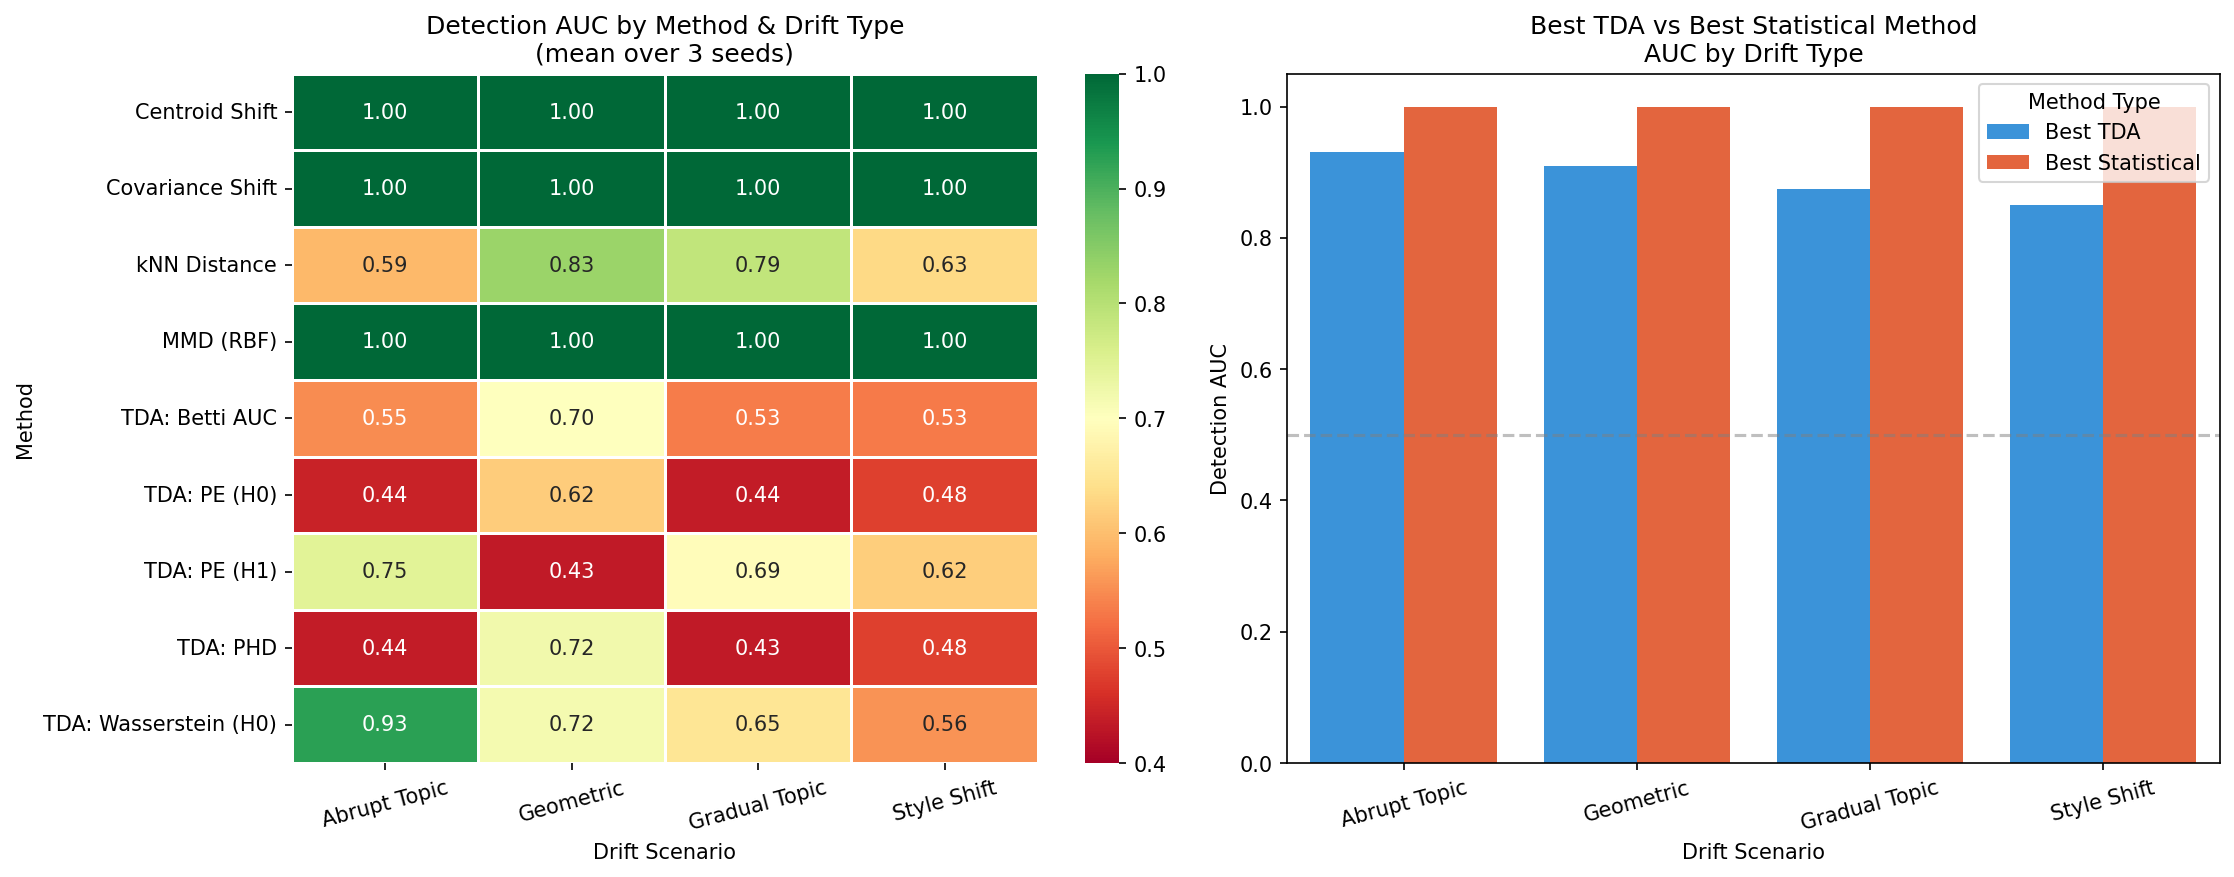
\includegraphics[width=0.95\linewidth]{figures/fig1_detection_by_drift_type.png}
    \caption{Detection AUC heatmap by method and drift type. Statistical methods (top three rows) achieve uniform AUC\,=\,1.0 across all scenarios. TDA methods show variable performance, with Wasserstein H0 performing best overall.}
    \label{fig:heatmap}
\end{figure}

\begin{figure}[t]
    \centering
    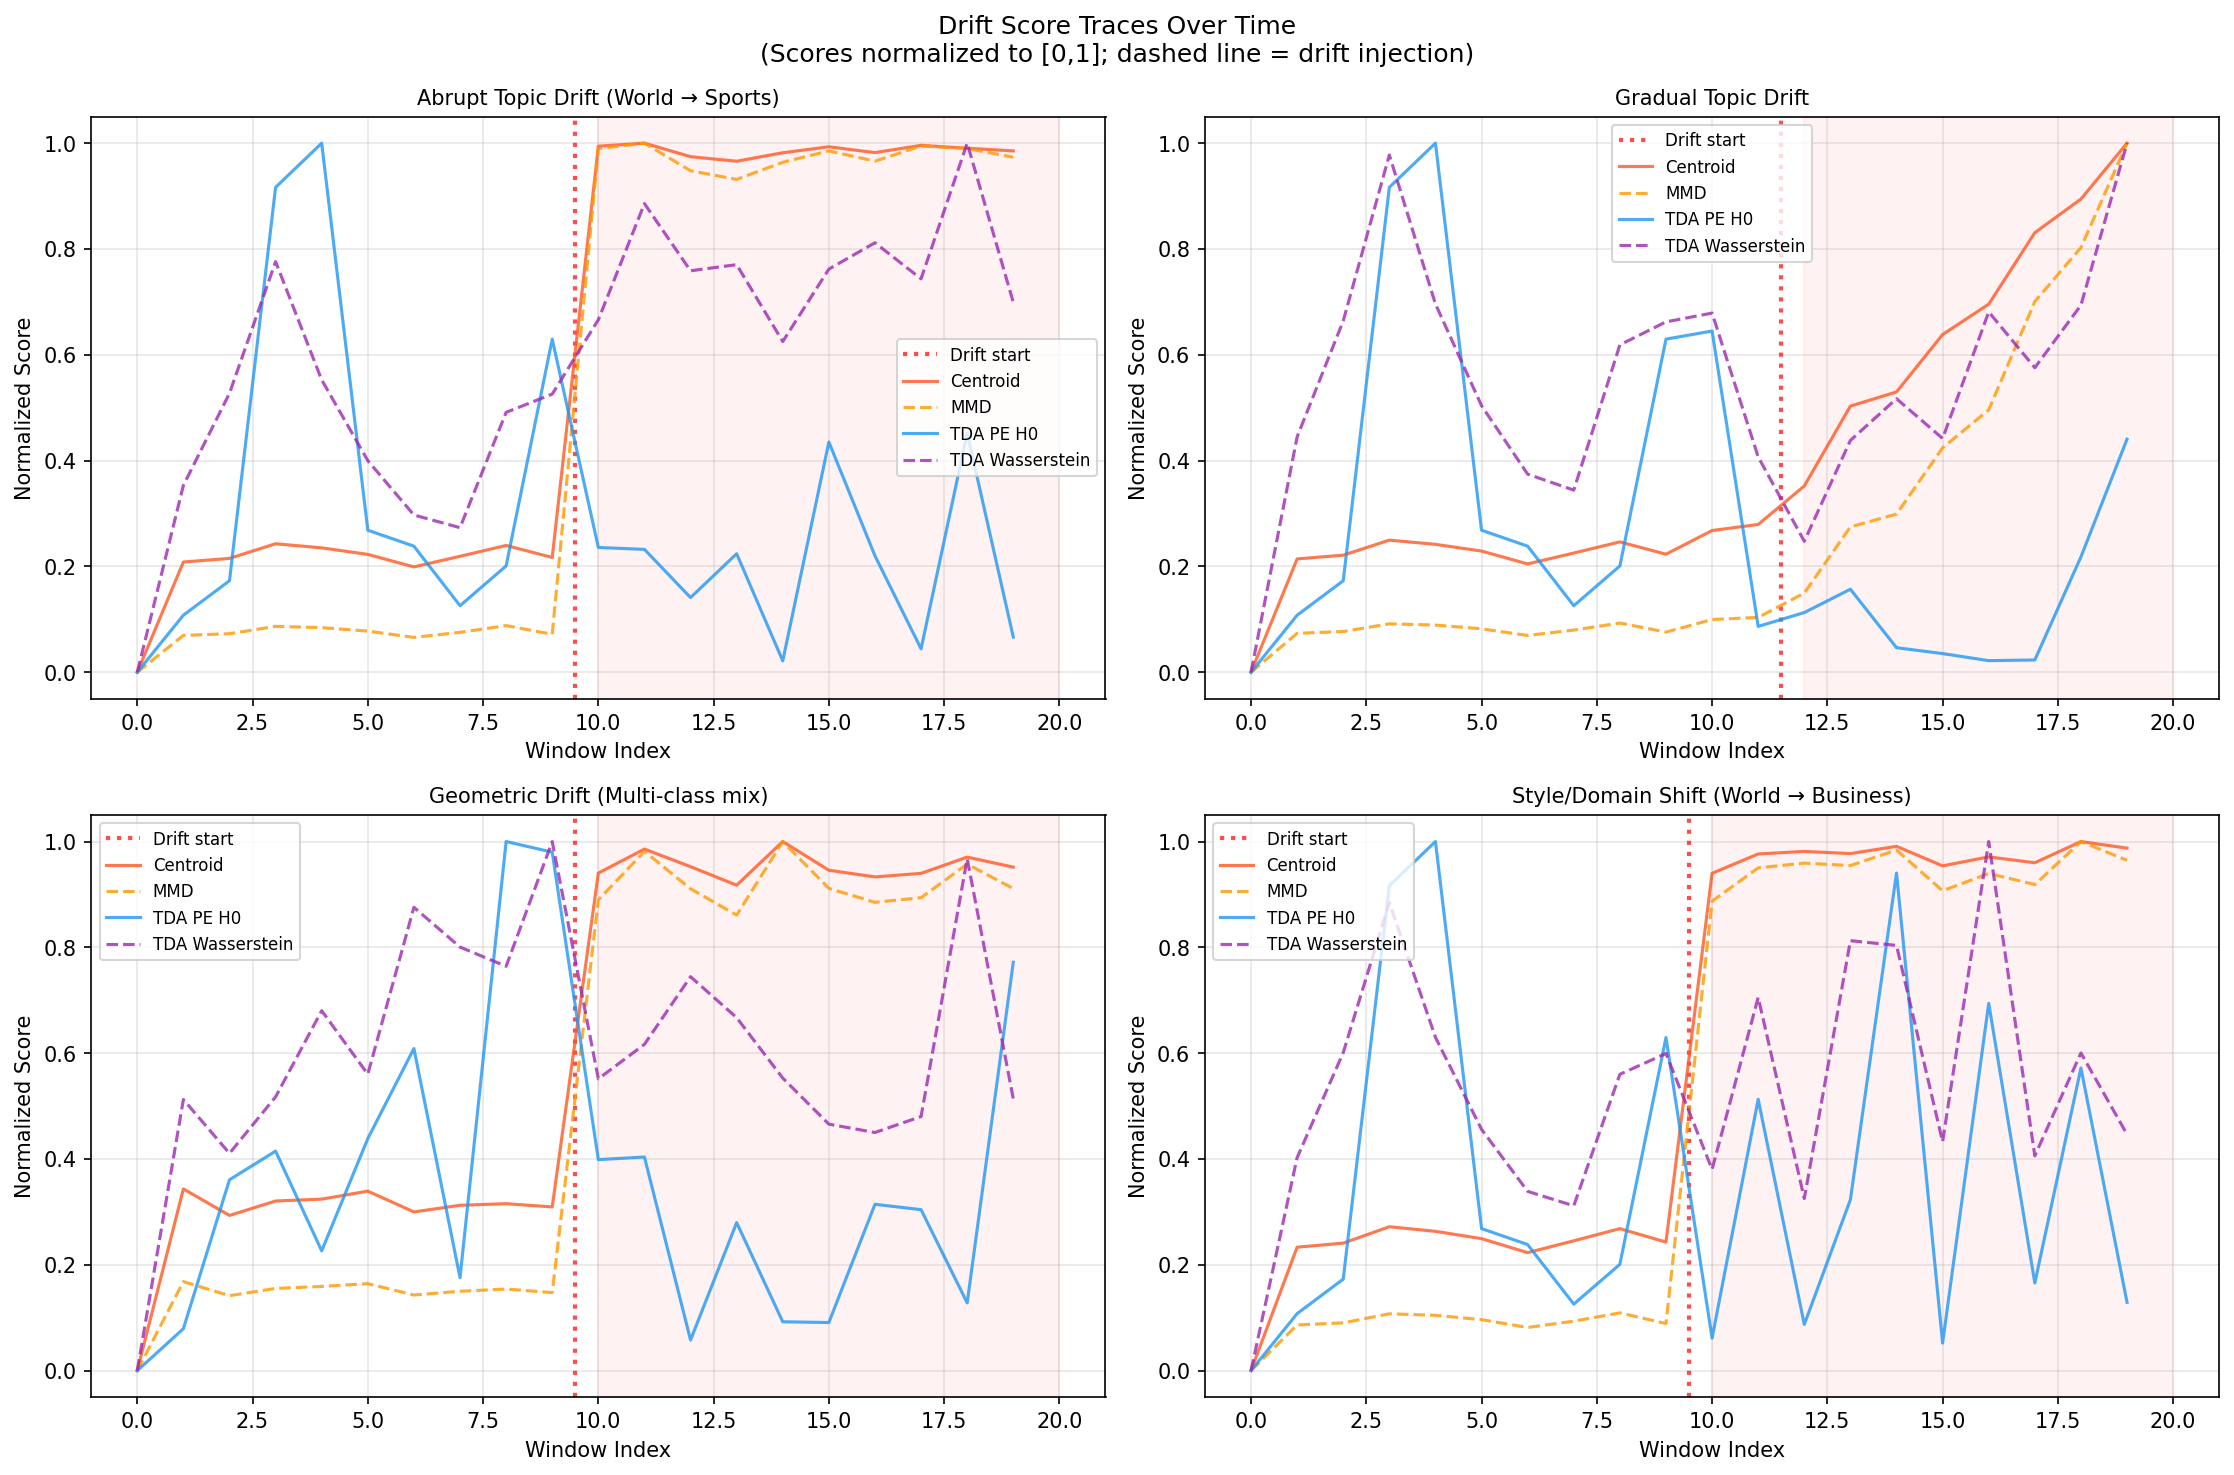
\includegraphics[width=0.95\linewidth]{figures/fig6_score_traces.png}
    \caption{Drift score traces over streaming windows. Statistical detectors produce sharp transitions at drift onset (vertical dashed line), while TDA scores exhibit higher variance and more gradual responses.}
    \label{fig:traces}
\end{figure}

\subsection{Synthetic Experiment: Topology-Only Drift}
\label{sec:synthetic_results}

\Tabref{tab:synthetic} presents separability ratios from the synthetic experiment, where higher values indicate stronger discrimination between drift and no-drift conditions. On centroid drift (positive control), MMD achieves the highest separability ($23.5\times$), followed by centroid shift ($7.6\times$). On loop drift---the key topology-preserving scenario---PE-H1 achieves $12.3\times$ separability, far exceeding centroid shift ($0.8\times$), which fails entirely. MMD also detects loop drift ($8.3\times$) but provides less interpretable signals. On split drift, MMD again leads ($6.5\times$), with TDA methods showing moderate sensitivity.

\begin{table}[t]
    \centering
    \caption{Separability ratio (drift score / no-drift score) on synthetic topology-only drift in 10 dimensions. Higher is better. PE-H1 uniquely detects loop drift ($\mathbf{12.3\times}$) where centroid shift fails ($0.8\times$).}
    \resizebox{\textwidth}{!}{%
    \begin{tabular}{@{}lcccccc@{}}
        \toprule
        & \multicolumn{3}{c}{\textbf{Statistical}} & \multicolumn{3}{c}{\textbf{TDA}} \\
        \cmidrule(lr){2-4} \cmidrule(lr){5-7}
        \textbf{Scenario} & Centroid & Cov & MMD & PE-H0 & \textbf{PE-H1} & Wass-H1 \\
        \midrule
        Centroid drift & 7.6$\times$ & 1.0$\times$ & \textbf{23.5$\times$} & 1.0$\times$ & 1.0$\times$ & 1.0$\times$ \\
        Loop (annulus) & 0.8$\times$ & 2.2$\times$ & 8.3$\times$ & 0.8$\times$ & \textbf{12.3$\times$} & 2.0$\times$ \\
        Split (2-cluster) & 0.7$\times$ & 2.0$\times$ & \textbf{6.5$\times$} & 1.2$\times$ & 1.6$\times$ & 2.4$\times$ \\
        \bottomrule
    \end{tabular}
    }
    \label{tab:synthetic}
\end{table}

\Figref{fig:synthetic} visualizes the synthetic experiment, showing point cloud configurations and detector responses for each drift type.

\begin{figure}[t]
    \centering
    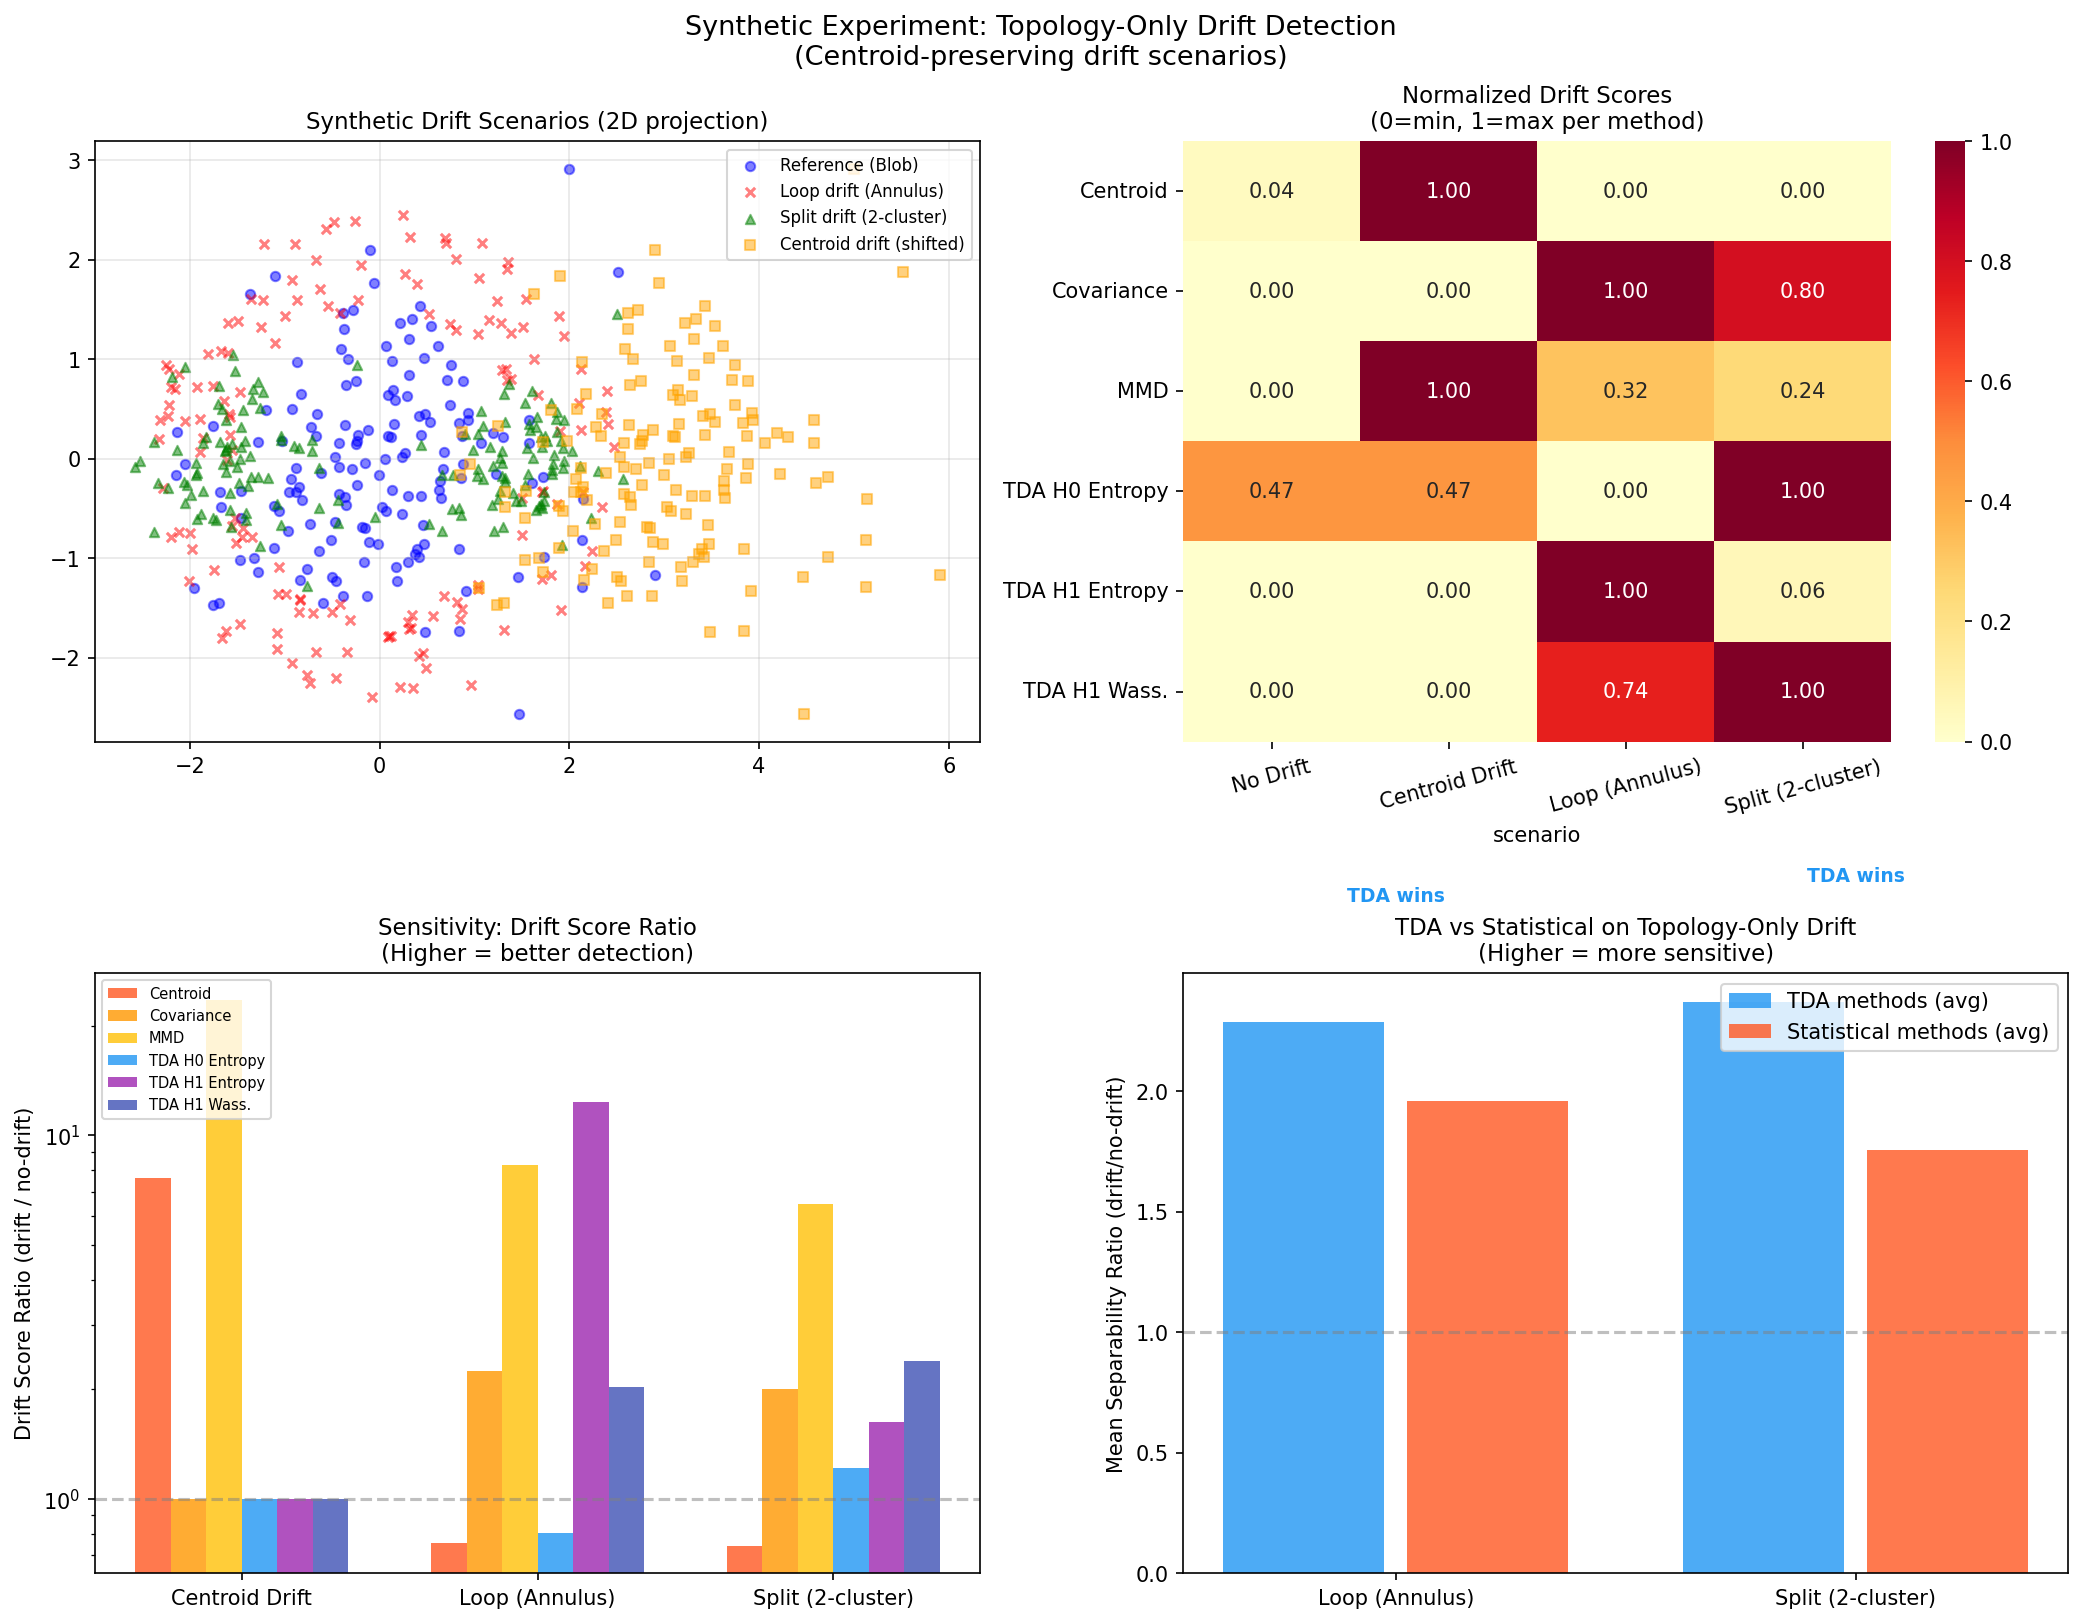
\includegraphics[width=0.95\linewidth]{figures/fig7_synthetic_topology_experiment.png}
    \caption{Synthetic topology-only drift experiment. \figleft Point cloud configurations for reference (Gaussian blob) and three drift types (centroid shift, annulus, two-cluster). \figright Separability ratios for each detector, showing PE-H1's unique advantage on loop drift.}
    \label{fig:synthetic}
\end{figure}

\subsection{Computational Cost}
\label{sec:runtime}

\Tabref{tab:runtime} summarizes runtime per window. Centroid shift is the fastest at 0.1ms. TDA methods occupy a middle ground: Wasserstein H0 runs in 2ms (the fastest TDA method) and full TDA computation (H0+H1 via \texttt{ripser}) takes $\sim$37ms---faster than both covariance shift (242ms) and MMD (126ms). All methods are operationally feasible for sub-second monitoring latency on CPU.

\begin{table}[t]
    \centering
    \caption{Runtime per 200-sample window on CPU. TDA methods are faster than covariance shift and MMD, occupying a computational middle ground.}
    \begin{tabular}{@{}lcc@{}}
        \toprule
        \textbf{Method} & \textbf{Runtime} & \textbf{Relative cost} \\
        \midrule
        Centroid Shift & 0.1ms & 1$\times$ \\
        kNN Distance & 31ms & 310$\times$ \\
        TDA (ripser H0) & 37ms & 370$\times$ \\
        Wasserstein H0 & 2ms & 20$\times$ \\
        MMD (RBF) & 126ms & 1{,}260$\times$ \\
        Covariance Shift & 242ms & 2{,}420$\times$ \\
        \bottomrule
    \end{tabular}
    \label{tab:runtime}
\end{table}

\subsection{Reproducibility Across Seeds}
\label{sec:reproducibility}

Statistical methods exhibit zero variance across seeds (std\,=\,0.000). TDA methods show higher variance: Wasserstein H0 has mean AUC\,=\,$0.713 \pm 0.192$ and PE-H1 has mean AUC\,=\,$0.624 \pm 0.215$, indicating greater sensitivity to sampling randomness in window subsampling.
